% \documentclass[a4paper,UKenglish,cleveref, autoref]{lipics-v2019}
\documentclass[12pt]{article}
\title{The Impact of Immutability on Class Size}
\author{Yegor Bugayenko}{}{}
% \authorrunning{Yegor Bugayenko}
% \ccsdesc[100]{Software and its engineering~Object oriented languages}
% \keywords{Object-Oriented Programming, Immutability, NCSS}
\usepackage[utf8]{inputenc}
\usepackage[numbers]{natbib}
\bibliographystyle{plainnat}
\usepackage[inline]{enumitem}
\usepackage{amsmath}
\usepackage{graphicx}
\usepackage{pgfplots}
\usepackage{verbatimbox}
\usepackage{interval}
\usepackage{hyperref}
\usepackage{minted}
  \setminted{fontsize=\footnotesize}
  \setminted{breaklines}
  \usemintedstyle{bw}
\newcommand{\code}[1]{\texttt{#1}}
\newenvironment{nicetable}
  {\setlength{\parindent}{0em}\medskip\small}
  {\medskip}
\def\thetotaljavafiles{97508}
\def\thetotalrepos{240}
\def\thelargestncss{34212}
\def\thebelowhundred{78304}

\begin{document}
\raggedbottom
\maketitle

\begin{abstract}
According to subjective opinions of many industry experts,
object immutability is a virtue in object-oriented programming, since it
leads to side-effect free design, cleaner code, better concurrency,
and many other factors. However, it has never been empirically
demonstrated exactly how immutability affects quality metrics of
object-oriented program. In the following research we analyzed
\thetotaljavafiles{} classes from \thetotalrepos{} public Java repositories
to find out how immutability affects the size of code.
\end{abstract}

\section{Introduction}

On one hand, one of the most important factors negatively affecting the quality
of object-oriented software is the \emph{size} of classes, as was
demonstrated by~\citet{li1993,al2013}: classes with lower size have better maintainability.
One of the simplest way
to calculate the size of a Java class is via the NCSS metric, which
stands for Non-Commenting Source Statements. Larger classes with bigger
amount of statements demonstrate higher values of NCSS.

On the other hand, \emph{immutability} is a property of a class in OOP. A class is immutable if
it's impossible to modify its attributes after instantiation. In Java this
technically means that all attributes have \texttt{final} modifier attached
to them.
Immutable classes greatly simplify programming, program maintenance, and
reasoning about programs. Immutable classes can be freely shared, even between
concurrent threads and with untrusted code, without the need to worry
about modifications, even temporary ones, that could result in
inconsistent states or broken invariants.
Immutability is a recommended coding practice for Java~\citep{bloch2016}.

This research empirically validates the relationship between immutability
and class size.

\section{Related Work}

Object immutability has been the subject of multiple researches since
the begining of object-oriented programming~\citep{hakonen1999,porat2000,lea2000,taivalsaari1993}.
Even though, according to~\citet{potanin2013},
``the notion of immutability is not as straightforward as it might seem, and many
different definitions of immutability exist,'' most industry experts consider
immutability being a virtue of classes and objects in Java and other
object-oriented programming languages~\citep{bloch2016}. There a few important
concerns of immutability addresses so far by object-oriented researchers.

First, even though Java encourages programmers to explicitly make objects immutable
by attaching the \texttt{final} modifier to its attributes, very often, as was
demonstrated by~\citet{unkel2008}, the modifier is not used even when
attributes are not modified after object instantiation or, as demonstrated
by~\citet{nelson2012}, after initialization. Such a delayed initialization of attributes, as
explained by~\citet{fahndrich2007}, leads to the prevalence of \texttt{null}
and the ability to initialize circular data structures, while both of these
practices have negative impact on software quality.

Second, despite the existence of the \texttt{final} modifier, Reflection API enables
modification of any attributes in Java. Some mechanisms were suggested to
overcome this technical vulnerability, for example
via ``freezer'' objects~\citep{leino2008},
a new type system~\citep{tschantz2005},
or immutability assertion framework~\citep{pechtchanski2005}.
However, without any modifications to Java~\citep{steele2005},
thanks to the existence of Reflection API,
it's not possible to say whether a particular Java object is modified
after instantiation or not---any object can be modified. As was noticed
by~\citet{hakonen1999} in relation to immutability,
``none of the current OO languages can prevent the programmer from writing
a piece of code which violates the integrity of an object''

Third, aside from the \texttt{final} modifier, which is an explicit way of declaring
read-only status of an attribute, there are also methods of
code analysis, enabling the detection of implicit immutability. For example,
a static flow-sensitive analysis algorithm was introduced by~\citet{porat2000}
to classify fields and classes as either mutable or immutable.

Forth, even if programmers do not violate encapsulation via reflection, the
modified \texttt{final} only guarantees shallow immutability, as
explained by~\citet{hakonen1999}. Deep immutability, on the other hand,
exists only if the object pointed by the attributes are deeply immutable
(recursively).

However, to our knowledge, the impact of immutability of class size has not been
analyzed yet.

\section{Empirical Results}

A list of Java repositories were retrieved from GitHub via their
public API. The first \thetotalrepos{} repositories were taken, which satisfied
the selection criteria:
\begin{enumerate*}[label={\arabic*)}]
\item more than 1,000 GitHub stars,
\item more than 200 Kb of data,
\item not archived, and
\item public.
\end{enumerate*}
The list included popular Java open source products, such as
Spring, RxJava, Guava, MyBatis, Clojure, JUnit, Lombok,
Graal, Selenium, Spark, Mockito, Neo4j, Jenkins, Netty, and others.

Files with \texttt{.java} extension were taken from all repositories.
There were \thetotaljavafiles{} files found. Classes without a single
non-\texttt{static} attribute were excluded (such as utility classes,
interfaces, or enums), despite the fact that some OOP
experts consider such classes valid and immutable, saying that
``the simplest immutable objects have no internal fields at all''~\citep{lea2000}.
We decided to not take these classes into account because they do not instantiate objects
and because of that do not belong to object-oriented paradigm,
as explained by~\cite{west2004,bugayenko2017}.

NCSS metric and immutability were calculated for each Java class,
using \texttt{javalang}, an open source Java-parsing library written in Python.
A class was considered immutable if it didn't have any
attributes without \texttt{final} modifier.

The Figure~\ref{fig:1} demonstrates the results obtained. The x-axis is
the value of NCSS of Java classes. The y-axis is the share of immutable classes among
all classes with the given NCSS. The diameter of the plot on the graph
is related to the amount of classes found for the specific NCSS. Classes
with NCSS larger than 1000 were excluded from the graph. This decision was
motivated by the confounding effect the size of a class has
on the validity of object-oriented metrics, as was empirically shown by~\citet{el2001}.
The right side of the graph has mostly (over 90\%) mutable classes. The largest
value of NCSS observed was \thelargestncss{}.

\begin{figure}[h]
  % Max: 3311
% Lo: 2
% Hi: 1000
% Step: 9.98 (steps: 100)
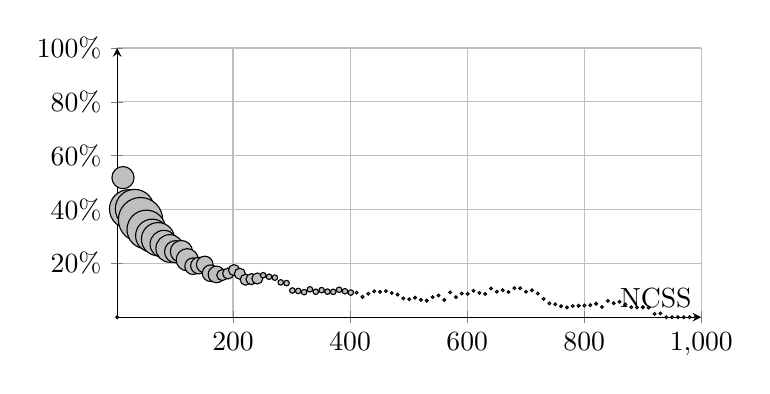
\begin{tikzpicture}
\begin{axis}[width=9cm,height=5cm,
axis lines=middle, xlabel={NCSS}, ylabel={},
xmin=2, xmax=1000, ymin=0, ymax=100,
yticklabel={\pgfmathprintnumber{\tick}\%},
extra tick style={major grid style=black},grid=major]
\addplot [only marks, mark=*, mark options={fill=lightgray,draw=black}, mark size=0.5pt] coordinates {
(2.0,0)};
\addplot [only marks, mark=*, mark options={fill=lightgray,draw=black}, mark size=4pt] coordinates {
(11.98,51.86260280599904)};
\addplot [only marks, mark=*, mark options={fill=lightgray,draw=black}, mark size=7pt] coordinates {
(21.96,40.19230769230769)};
\addplot [only marks, mark=*, mark options={fill=lightgray,draw=black}, mark size=7pt] coordinates {
(31.94,40.29714978775015)};
\addplot [only marks, mark=*, mark options={fill=lightgray,draw=black}, mark size=8pt] coordinates {
(41.92,36.24282694050136)};
\addplot [only marks, mark=*, mark options={fill=lightgray,draw=black}, mark size=7pt] coordinates {
(51.900000000000006,32.57948213700426)};
\addplot [only marks, mark=*, mark options={fill=lightgray,draw=black}, mark size=6pt] coordinates {
(61.88,30.265995686556437)};
\addplot [only marks, mark=*, mark options={fill=lightgray,draw=black}, mark size=6pt] coordinates {
(71.86,28.994082840236686)};
\addplot [only marks, mark=*, mark options={fill=lightgray,draw=black}, mark size=5pt] coordinates {
(81.84,27.139874739039666)};
\addplot [only marks, mark=*, mark options={fill=lightgray,draw=black}, mark size=5pt] coordinates {
(91.82000000000001,25.547445255474454)};
\addplot [only marks, mark=*, mark options={fill=lightgray,draw=black}, mark size=4pt] coordinates {
(101.80000000000001,24.345679012345677)};
\addplot [only marks, mark=*, mark options={fill=lightgray,draw=black}, mark size=4pt] coordinates {
(111.78,24.395604395604394)};
\addplot [only marks, mark=*, mark options={fill=lightgray,draw=black}, mark size=4pt] coordinates {
(121.76,21.356502242152466)};
\addplot [only marks, mark=*, mark options={fill=lightgray,draw=black}, mark size=3pt] coordinates {
(131.74,18.953846153846154)};
\addplot [only marks, mark=*, mark options={fill=lightgray,draw=black}, mark size=3pt] coordinates {
(141.72,19.180887372013654)};
\addplot [only marks, mark=*, mark options={fill=lightgray,draw=black}, mark size=3pt] coordinates {
(151.70000000000002,19.58997722095672)};
\addplot [only marks, mark=*, mark options={fill=lightgray,draw=black}, mark size=3pt] coordinates {
(161.68,16.338880484114977)};
\addplot [only marks, mark=*, mark options={fill=lightgray,draw=black}, mark size=3pt] coordinates {
(171.66,15.89825119236884)};
\addplot [only marks, mark=*, mark options={fill=lightgray,draw=black}, mark size=2pt] coordinates {
(181.64000000000001,15.646258503401361)};
\addplot [only marks, mark=*, mark options={fill=lightgray,draw=black}, mark size=2pt] coordinates {
(191.62,16.25794732061762)};
\addplot [only marks, mark=*, mark options={fill=lightgray,draw=black}, mark size=2pt] coordinates {
(201.60000000000002,17.51412429378531)};
\addplot [only marks, mark=*, mark options={fill=lightgray,draw=black}, mark size=2pt] coordinates {
(211.58,16.151545363908276)};
\addplot [only marks, mark=*, mark options={fill=lightgray,draw=black}, mark size=2pt] coordinates {
(221.56,13.934426229508196)};
\addplot [only marks, mark=*, mark options={fill=lightgray,draw=black}, mark size=2pt] coordinates {
(231.54000000000002,14.146868250539956)};
\addplot [only marks, mark=*, mark options={fill=lightgray,draw=black}, mark size=2pt] coordinates {
(241.52,14.387633769322235)};
\addplot [only marks, mark=*, mark options={fill=lightgray,draw=black}, mark size=1pt] coordinates {
(251.5,15.590742996345918)};
\addplot [only marks, mark=*, mark options={fill=lightgray,draw=black}, mark size=1pt] coordinates {
(261.48,15.031847133757962)};
\addplot [only marks, mark=*, mark options={fill=lightgray,draw=black}, mark size=1pt] coordinates {
(271.46000000000004,14.701803051317613)};
\addplot [only marks, mark=*, mark options={fill=lightgray,draw=black}, mark size=1pt] coordinates {
(281.44,12.949640287769784)};
\addplot [only marks, mark=*, mark options={fill=lightgray,draw=black}, mark size=1pt] coordinates {
(291.42,12.669683257918551)};
\addplot [only marks, mark=*, mark options={fill=lightgray,draw=black}, mark size=1pt] coordinates {
(301.40000000000003,9.923664122137405)};
\addplot [only marks, mark=*, mark options={fill=lightgray,draw=black}, mark size=1pt] coordinates {
(311.38,9.748427672955975)};
\addplot [only marks, mark=*, mark options={fill=lightgray,draw=black}, mark size=1pt] coordinates {
(321.36,9.317803660565724)};
\addplot [only marks, mark=*, mark options={fill=lightgray,draw=black}, mark size=1pt] coordinates {
(331.34000000000003,10.35120147874307)};
\addplot [only marks, mark=*, mark options={fill=lightgray,draw=black}, mark size=1pt] coordinates {
(341.32,9.454545454545455)};
\addplot [only marks, mark=*, mark options={fill=lightgray,draw=black}, mark size=1pt] coordinates {
(351.3,10.054844606946983)};
\addplot [only marks, mark=*, mark options={fill=lightgray,draw=black}, mark size=1pt] coordinates {
(361.28000000000003,9.496124031007753)};
\addplot [only marks, mark=*, mark options={fill=lightgray,draw=black}, mark size=1pt] coordinates {
(371.26,9.421841541755889)};
\addplot [only marks, mark=*, mark options={fill=lightgray,draw=black}, mark size=1pt] coordinates {
(381.24,10.199556541019955)};
\addplot [only marks, mark=*, mark options={fill=lightgray,draw=black}, mark size=1pt] coordinates {
(391.22,9.647058823529411)};
\addplot [only marks, mark=*, mark options={fill=lightgray,draw=black}, mark size=1pt] coordinates {
(401.20000000000005,9.156626506024097)};
\addplot [only marks, mark=*, mark options={fill=lightgray,draw=black}, mark size=0.5pt] coordinates {
(411.18,9.135802469135802)};
\addplot [only marks, mark=*, mark options={fill=lightgray,draw=black}, mark size=0.5pt] coordinates {
(421.16,7.567567567567568)};
\addplot [only marks, mark=*, mark options={fill=lightgray,draw=black}, mark size=0.5pt] coordinates {
(431.14000000000004,8.743169398907105)};
\addplot [only marks, mark=*, mark options={fill=lightgray,draw=black}, mark size=0.5pt] coordinates {
(441.12,9.63855421686747)};
\addplot [only marks, mark=*, mark options={fill=lightgray,draw=black}, mark size=0.5pt] coordinates {
(451.1,9.433962264150944)};
\addplot [only marks, mark=*, mark options={fill=lightgray,draw=black}, mark size=0.5pt] coordinates {
(461.08000000000004,9.67741935483871)};
\addplot [only marks, mark=*, mark options={fill=lightgray,draw=black}, mark size=0.5pt] coordinates {
(471.06,9.0)};
\addplot [only marks, mark=*, mark options={fill=lightgray,draw=black}, mark size=0.5pt] coordinates {
(481.04,8.411214953271028)};
\addplot [only marks, mark=*, mark options={fill=lightgray,draw=black}, mark size=0.5pt] coordinates {
(491.02000000000004,7.006369426751593)};
\addplot [only marks, mark=*, mark options={fill=lightgray,draw=black}, mark size=0.5pt] coordinates {
(501.0,6.666666666666667)};
\addplot [only marks, mark=*, mark options={fill=lightgray,draw=black}, mark size=0.5pt] coordinates {
(510.98,7.241379310344828)};
\addplot [only marks, mark=*, mark options={fill=lightgray,draw=black}, mark size=0.5pt] coordinates {
(520.96,6.474820143884892)};
\addplot [only marks, mark=*, mark options={fill=lightgray,draw=black}, mark size=0.5pt] coordinates {
(530.94,6.172839506172839)};
\addplot [only marks, mark=*, mark options={fill=lightgray,draw=black}, mark size=0.5pt] coordinates {
(540.9200000000001,7.456140350877193)};
\addplot [only marks, mark=*, mark options={fill=lightgray,draw=black}, mark size=0.5pt] coordinates {
(550.9,8.071748878923767)};
\addplot [only marks, mark=*, mark options={fill=lightgray,draw=black}, mark size=0.5pt] coordinates {
(560.88,6.422018348623854)};
\addplot [only marks, mark=*, mark options={fill=lightgray,draw=black}, mark size=0.5pt] coordinates {
(570.86,9.251101321585903)};
\addplot [only marks, mark=*, mark options={fill=lightgray,draw=black}, mark size=0.5pt] coordinates {
(580.84,7.456140350877193)};
\addplot [only marks, mark=*, mark options={fill=lightgray,draw=black}, mark size=0.5pt] coordinates {
(590.82,8.81057268722467)};
\addplot [only marks, mark=*, mark options={fill=lightgray,draw=black}, mark size=0.5pt] coordinates {
(600.8000000000001,8.695652173913043)};
\addplot [only marks, mark=*, mark options={fill=lightgray,draw=black}, mark size=0.5pt] coordinates {
(610.78,9.813084112149532)};
\addplot [only marks, mark=*, mark options={fill=lightgray,draw=black}, mark size=0.5pt] coordinates {
(620.76,9.047619047619047)};
\addplot [only marks, mark=*, mark options={fill=lightgray,draw=black}, mark size=0.5pt] coordinates {
(630.74,8.653846153846153)};
\addplot [only marks, mark=*, mark options={fill=lightgray,draw=black}, mark size=0.5pt] coordinates {
(640.72,10.65989847715736)};
\addplot [only marks, mark=*, mark options={fill=lightgray,draw=black}, mark size=0.5pt] coordinates {
(650.7,9.473684210526317)};
\addplot [only marks, mark=*, mark options={fill=lightgray,draw=black}, mark size=0.5pt] coordinates {
(660.6800000000001,10.05586592178771)};
\addplot [only marks, mark=*, mark options={fill=lightgray,draw=black}, mark size=0.5pt] coordinates {
(670.6600000000001,9.35672514619883)};
\addplot [only marks, mark=*, mark options={fill=lightgray,draw=black}, mark size=0.5pt] coordinates {
(680.64,10.828025477707007)};
\addplot [only marks, mark=*, mark options={fill=lightgray,draw=black}, mark size=0.5pt] coordinates {
(690.62,10.738255033557047)};
\addplot [only marks, mark=*, mark options={fill=lightgray,draw=black}, mark size=0.5pt] coordinates {
(700.6,9.45945945945946)};
\addplot [only marks, mark=*, mark options={fill=lightgray,draw=black}, mark size=0.5pt] coordinates {
(710.58,10.0)};
\addplot [only marks, mark=*, mark options={fill=lightgray,draw=black}, mark size=0.5pt] coordinates {
(720.5600000000001,8.823529411764707)};
\addplot [only marks, mark=*, mark options={fill=lightgray,draw=black}, mark size=0.5pt] coordinates {
(730.5400000000001,6.8181818181818175)};
\addplot [only marks, mark=*, mark options={fill=lightgray,draw=black}, mark size=0.5pt] coordinates {
(740.52,5.147058823529411)};
\addplot [only marks, mark=*, mark options={fill=lightgray,draw=black}, mark size=0.5pt] coordinates {
(750.5,4.794520547945205)};
\addplot [only marks, mark=*, mark options={fill=lightgray,draw=black}, mark size=0.5pt] coordinates {
(760.48,4.081632653061225)};
\addplot [only marks, mark=*, mark options={fill=lightgray,draw=black}, mark size=0.5pt] coordinates {
(770.46,3.64963503649635)};
\addplot [only marks, mark=*, mark options={fill=lightgray,draw=black}, mark size=0.5pt] coordinates {
(780.44,4.166666666666666)};
\addplot [only marks, mark=*, mark options={fill=lightgray,draw=black}, mark size=0.5pt] coordinates {
(790.4200000000001,4.25531914893617)};
\addplot [only marks, mark=*, mark options={fill=lightgray,draw=black}, mark size=0.5pt] coordinates {
(800.4000000000001,4.316546762589928)};
\addplot [only marks, mark=*, mark options={fill=lightgray,draw=black}, mark size=0.5pt] coordinates {
(810.38,4.477611940298507)};
\addplot [only marks, mark=*, mark options={fill=lightgray,draw=black}, mark size=0.5pt] coordinates {
(820.36,5.0)};
\addplot [only marks, mark=*, mark options={fill=lightgray,draw=black}, mark size=0.5pt] coordinates {
(830.34,3.8095238095238098)};
\addplot [only marks, mark=*, mark options={fill=lightgray,draw=black}, mark size=0.5pt] coordinates {
(840.32,6.0606060606060606)};
\addplot [only marks, mark=*, mark options={fill=lightgray,draw=black}, mark size=0.5pt] coordinates {
(850.3000000000001,5.208333333333334)};
\addplot [only marks, mark=*, mark options={fill=lightgray,draw=black}, mark size=0.5pt] coordinates {
(860.2800000000001,5.747126436781609)};
\addplot [only marks, mark=*, mark options={fill=lightgray,draw=black}, mark size=0.5pt] coordinates {
(870.26,4.761904761904762)};
\addplot [only marks, mark=*, mark options={fill=lightgray,draw=black}, mark size=0.5pt] coordinates {
(880.24,3.7037037037037033)};
\addplot [only marks, mark=*, mark options={fill=lightgray,draw=black}, mark size=0.5pt] coordinates {
(890.22,3.614457831325301)};
\addplot [only marks, mark=*, mark options={fill=lightgray,draw=black}, mark size=0.5pt] coordinates {
(900.2,3.7037037037037033)};
\addplot [only marks, mark=*, mark options={fill=lightgray,draw=black}, mark size=0.5pt] coordinates {
(910.1800000000001,3.571428571428571)};
\addplot [only marks, mark=*, mark options={fill=lightgray,draw=black}, mark size=0.5pt] coordinates {
(920.1600000000001,1.25)};
\addplot [only marks, mark=*, mark options={fill=lightgray,draw=black}, mark size=0.5pt] coordinates {
(930.14,1.4084507042253522)};
\addplot [only marks, mark=*, mark options={fill=lightgray,draw=black}, mark size=0.5pt] coordinates {
(940.12,0.0)};
\addplot [only marks, mark=*, mark options={fill=lightgray,draw=black}, mark size=0.5pt] coordinates {
(950.1,0.0)};
\addplot [only marks, mark=*, mark options={fill=lightgray,draw=black}, mark size=0.5pt] coordinates {
(960.08,0.0)};
\addplot [only marks, mark=*, mark options={fill=lightgray,draw=black}, mark size=0.5pt] coordinates {
(970.0600000000001,0.0)};
\addplot [only marks, mark=*, mark options={fill=lightgray,draw=black}, mark size=0.5pt] coordinates {
(980.0400000000001,0.0)};
\addplot [only marks, mark=*, mark options={fill=lightgray,draw=black}, mark size=0.5pt] coordinates {
(990.0200000000001,0.0)};
\end{axis}\end{tikzpicture}

  \caption{Distribution of class immutability by NCSS}
  \label{fig:1}
\end{figure}

The tendency is visually obvious: larger classes are less often immutable. It
was also observed that the majority of classes have NCSS values smaller than 100:
\thebelowhundred{} classes out of \thetotaljavafiles{} total.

\section{Conclusion}

It was empirically confirmed that larger Java classes tend to be immutable
less frequently than smaller ones. At the same time it is possible to conclude
that immutable classes tend to be smaller. Both conclusions justify
the hypothesis that immutability in object-oriented programming leads
to higher maintainability, since classes will be smaller.

The source code of Ruby and Python scripts used to do the research
is available in GitHub repository \texttt{yegor256/size-vs-immutability}.

\bibliography{main}

\end{document}
